\section{Spineless Traversal}

Spineless traversal is a new algorithm
  for finding the dirty nodes in the layout tree.
At its core, spineless traversal recognizes
  that the main cost of the Double Dirty Bit algorithm
  is cache misses due to too many auxiliary nodes.
It therefore uses a more computationally-heavy approach
  to jump directly to dirty nodes instead of traversing the tree;
  this trades more computation for fewer cache misses
  and thus results in greater performance.

\subsection{The Priority Queue}

Spineless traversal is conceptually simple.
Each node field in the layout tree is assigned a label,
  indicating its position in the trace of a non-incremental layout.
Node fields are placed in a priority queue when dirtied,
  with the label used as their priority.
To perform an incremental layout,
  node fields are popped from the priority queue and recomputed,
  with dependent fields
  added back to the priority queue as they get dirtied,
  until the priority queue is empty.
Because the priority queue pops smaller node field labels first,
  a spineless traversal visits node fields in order
  and thus respects the dependency order of layout.

Since only dirty nodes are even pushed or popped from the priority queue,
  no auxiliary nodes are accessed.
This means that spineless traversal has the potential
  to dramatically speed up traversal,
  assuming the priority queue operations themselves
  don't add too much overhead.
We use a min-heap for our priority queue,
  which is cache-friendly and requires relatively few operations
  for each push and pop.
Moreover, the queue is typically small:
  while there are typically thousands of nodes,
  with each node having approximately 50 fields,
  the priority queue typically contains less then 1000 elements,
  and for the most latency-critical interactions,
  like hovers or drags, it can contain 100 elements or fewer.
With such a small size, a priority queue push/pop requires
  10--20 label comparisons,
  which can be performed in roughly the time
  for one or two L3 cache accesses
  in our optimized implementation.


\begin{figure}
\scalebox{0.7}{
\begin{forest}
  [body 
    [header [a] [div [nav [a] [a] [a] [a] [a]] [nav [a]]]]
    [div 
      [ol 
        [li 
          [div 
            [div [a] [div]] 
            [div 
              [span [a]] 
              [span [a] [a]]
              [a]
              [div 
                [a [img]] 
                [span]
                [a]
                [span]
                [span]
                [span [input] [label [div [a] [a, color=green, name=popped] [a, color=orange, name=pushed]]]] 
                [span [span] [a]]]]]]
        [a [span]]]
    [div]
    [ol
      [li
        [div
          [form
            [input]
            [input, color=yellow]
            [input
              [div
                [textarea
                  [p]
                  [div
                    [input] [button] [div]]]]
              [p]]]]]
      [li]]]
    [footer [a] [a] [a] [a]]
    [span]]
\draw[] (1,-11) rectangle (2,-12) node[pos=.5, color=green] {a};
\draw[->] (1.5, -11) to (popped);
\draw[] (2,-11) rectangle (3,-12) node[pos=.5, color=yellow] {input}; \draw[<-] (2, -11) to (pushed);
\end{forest}
}
\centering
\caption{Spineless Traversal instead store all elements in a priority queue, eschewing the need to traverse spine+1. The queue initially contain the green "a" and the yellow "input" node. In a single iteration, spineless traversal pop the green "a" off the queue and process it, which push the orange "a" into the queue, and it is inserted before the yellow "input" to respect the time order.}
% https://lobste.rs/s/7ixd88/c_complexity_compiler_bugs
\label{fig:dom-tree-pq}
\end{figure}

\subsection{Order Maintenance}

The labels themselves, however, are challenging to maintain.
The issue is that layout nodes are added and removed over time;
  labels need to be comparable,
  but it also needs to be possible
  to add new labels between existing ones,
  arbitrarily.
Following SAC~\cite{SAC},
  spineless traversal achieves this using
  the \emph{order maintenance} data structure.
First introduced by \citet{OM},
  order maintenance is a data structure
  that maintains a totally ordered set of objects
  while allowing objects
  to be added and removed from the order arbitrarily.
One can imagine order maintenance as a doubly-linked list,
  where nodes can be added and removed in $O(1)$ time;
  however, unlike a simple double-linked list,
  order maintenance also permits an $O(1)$ order comparison function.
Abstractly, order maintenance provides the following API:

\begin{enumerate}
\setlength{\itemindent}{8em}
  
\item[$\mathsf{Compare}(p, q)$] Decides whether $p$ or $q$ comes first in the order (or are equal).
\item[$\mathsf{Head}()$] Returns the first object of the list.
\item[$\mathsf{Create}(p)$] Creates and returns a new object right after $p$.
\end{enumerate}

\noindent
Deleting OM objects is also possible; however,
  our implementation does not use this method.
\todo{Maybe try implementing it}

Our implementation is based on that by \citet{SOM},
  % two simplified algorithm for linked list
  which uses a two-level structure with
  a double-linked list of double-linked lists.
Objects are represented by nodes in the lower-level lists;
  the total order can be recovered by flattening this structure,
  concatenating all lower-level lists
  in the order dictated by the higher-level list.
Each object (node in the lower-level list)
  maintains a pointer to its higher-level list cell;
  two objects are in the same low-level list
  if they have the same higher-level pointer.
Comparing two objects then has two cases:
  the two objects can be in the same low-level list,
  or in different ones.
To allow fast comparisons between nodes,
  both low-level and high-level list cells store
  an unsigned integer of fixed size
  (in our implementation, unsigned 32-bit integers)
  called labels.
Within a lower-level list,
  node labels are strictly increasing,
  making comparison fast.
Higher-level lists have the same invariant.

To create an object inside an order maintenance structure,
  a new lower-level list cell is created
  whose label is the average of the two neighboring labels.
\footnote{
  When creating a node after the last node,
  the maximum representable number is used as the larger number.
}
If the two labels differ by exactly 1, however,
  this becomes impossible (a label would be repeated).
In this case, the data structure re-balances itself,
  evenly reassigning labels to existing objects.
During relabeling, a new higher-level list cell might be created,
  and the lower-level list may be split in two,
  ensuring a sufficiently-large gap the elements.
Rebalancing is algorithmically tricky
  but is not a significant time sink in our use case,
  so we do not detail re-balancing here;
  details can be found in \citet{SOM}.

\begin{figure}
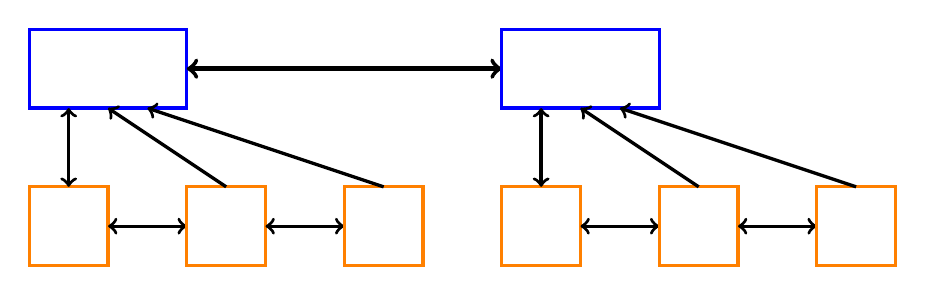
\begin{tikzpicture}
\draw[blue, very thick] (0,0) rectangle (2,1);
\draw[ultra thick, <->] (2,0.5) -- (6,0.5);
\draw[blue, very thick] (6,0) rectangle (8,1);

\draw[orange, very thick] (0, -2) rectangle (1,-1);
\draw[very thick, <->] (0.5,-1) -- (0.5,0);
\draw[very thick, <->] (1,-1.5) -- (2,-1.5);
\draw[orange, very thick] (2, -2) rectangle (3,-1);
\draw[very thick, ->] (2.5,-1) -- (1,0);
\draw[very thick, <->] (3,-1.5) -- (4,-1.5);
\draw[orange, very thick] (4, -2) rectangle (5,-1);
\draw[very thick, ->] (4.5,-1) -- (1.5,0);

\draw[orange, very thick] (6, -2) rectangle (7,-1);
\draw[very thick, <->] (6.5,-1) -- (6.5,0);
\draw[very thick, <->] (7,-1.5) -- (8,-1.5);
\draw[orange, very thick] (8,-2) rectangle (9,-1);
\draw[very thick, ->] (8.5,-1) -- (7,0);
\draw[very thick, <->] (9,-1.5) -- (10,-1.5);
\draw[orange, very thick] (10, -2) rectangle (11,-1);
\draw[very thick, ->] (10.5,-1) -- (7.5,0);

\end{tikzpicture}
\caption{An Order Maintenance data structure. The blue node represent the higher level doubly linked list, and each node store a lower level doubly linked list, denoted by the red node. Lower level node also store a pointer to the higher level node. Each node additionally hold an unsigned integer, label, such that inside a single list the node earlier have a strictly smaller label then the node later.}
\label{fig:om}
\end{figure}

\subsection{Bulk insertion and deletion}
Special care has to be taken to handle insertion or deletion
  of whole subtrees at a time;
  this is common in modern JavaScript applications built
  using ``virtual DOM'' frameworks such as JavaScript.

When the user interact with the webpage, the underlying javascript might decide to insert or delete a subtree. This subtree is then translated into a layout tree.
Inserting and deleting layout nodes
  ultimately requires creating and deleting
  order maintenance objects,
  but special care has to be taken to
  deal efficiently with subtrees.
\todo{Dependency: need to clarify that whole subtrees are inserted/deleted.}

When a subtree rooted at $r$ is inserted,
  the pair $(r, v)$ is pushed into the priority queue
  for each variable $v$ in the layout program.
The position of this pair must match
  its position in a trace of the layout program.
That is, it must come after $(n', v')$
  computed before $r.v$
  and before any $(n'', v'')$ computed after $r.v$.
To do so,
  spineless traversal creates a new order maintenance object
  after the last field, according to the order maintenance,
  in either the previous sibling or parent node of the new subtree.
Note that only the root of the inserted subtree
  needs to be pushed into the priority queue.
This is because, after visiting the root,
  the layout program will proceed to visit all its children,
  and so on recursively until the whole subtree has been visited.
\footnote{
  As a further edge case,
    it is possible that the subtree is inserted into
    a subtree that itself has not yet been laid out.
  In this case no further actions need to be taken,
    since both subtrees would be initialized in one go.}

Deleting a subtree is also challenging
  because some nodes in the subtree may already be in the priority queue;
  for example, this can happen if
  a subtree is inserted and then later deleted.
To avoid unnecessary recomputation,
  we add a ``deleted'' bit to each node
  instead of deallocating it immediately.
Recomputation is then skipped for deleted nodes,
  and the nodes are actually deallocated
  when a incremental layout is finished
  and the priority queue is empty.%
\footnote{Some browsers may choose
  to retain layout nodes even longer,
  or even to garbage-collect them.
}
